\section{State redistribution in two dimensions}\label{sec:srdAlg}

For simplicity, we restrict our description to the second order accurate state redistribution algorithm for scalar conservation laws.  A framework for extension to arbitrarily high order accuracy is presented in Appendix \ref{sec:ho}.  
%The extension to systems of conservation laws is direct and discussed at the start of Section \ref{sec:srd_postprocessing}.
%We first describe the second order accurate version of the state
%redistribution algorithm. 
%This helps simplify the notation and make the algorithm more intuitive.   
%At several places we discuss the alternatives and the reason behind our choices.  
%Then, we extend the state redistribution procedure in Section \ref{sec:srd1d} to two dimensional cut cell grids and second order accuracy in time and space.

\subsection{State redistribution preprocessing}\label{sec:preprocessing}


%In this section, we describe mesh dependent quantities that will be used in the second order accurate state redistribution method, i.e., the two-dimensional analogue of preprocessing on one-dimensional nonuniform grids presented in Section \ref{sec:srd1d}.
In this section, we describe preprocessing of mesh-dependent quantities on two-dimensional meshes with overlapping neighborhoods, i.e., the analogue of preprocessing on one-dimensional nonuniform grids presented in Section \ref{sec:srd1d}.

Preprocessing determines merging neighborhoods, weighted volumes and centroids.  These quantities only need to be computed once during a mesh preprocessing step since as will not vary over the course of a simulation.  
%We describe here the two dimensional analogue of Section \ref{sec:srd1d}, which describes preprocessing on a one dimensional nonuniform grid.

%, although for a moving geometry, 

%These three steps can be part of a preprocessing step since they do not
%depend on the computed solution. 
%However for moving geometry they would
%be done at each step.

\subsubsection*{Merging neighborhoods}

%\begin{itemize}
%\item
%{\bf Each cut cell finds adjacent cells to {\em temporarily} merge with.}

%\vspace*{.1in}

%On a regular grid of rectangles, it can be shown that the time step restriction for a local maximum principle satisfying scheme requires a CFL number of $\frac{1}{4}$ [].

In one dimension, neighborhoods can be defined by merging a small cell with neighbors on its left, on its right, or both.  Of these three approaches, the last was used on the nonuniform grid presented in Section \ref{sec:srd1d},
In two dimensions, there is much more freedom in defining a merging neighborhood.  Here, we propose two different ways: (1) normal merging and (2) centered merging.

Normal merging associates cut cells with neighbors in the direction closest to the 
boundary normal.  This is illustrated in Figure \ref{fig:neighborhoods}, where the normal merging neighborhood associated to cut cell $(i,j)$ is highlighted in green.

Centered merging associates cut cells with neighbors that are at most e.g. one cell away, that is, cells located on the $3 \times 3$ tile centered on the small cell.  This is illustrated in Figure \ref{fig:neighborhoods}, where the centered tile merging neighborhood associated to cut cell $(i+3,j+1)$ is highlighted in green.


The larger the neighborhood the more diffusive the results, thus we do not want neighborhoods that are too large.  However, they must satisfy a size constraint to dampen unstable growth in the numerical solution. To this end, we determine neighborhoods, either normal or centered, such that the
volume of the neighborhood is at least half the area of an uncut cell, i.e., 
\begin{equation} \label{eqn:vmerge}
\sum_{(r,s) \in M_{i,j}} V_{r,s} \geq \frac{1}{2}\Delta x \Delta y,
\end{equation}
where $M_{i,j}$ denotes the set of cell indices that belong to 
merging neighborhood $(i,j)$.    
The threshold of $1/2$ the area of a full has been shown in one dimension \cite{mjb:stability2} to be 
sufficient for stability.  We have not encountered any issues with this choice in two dimensions.
% with several schemes whose stability limit is $\le 1$

For smooth solutions a centered neighborhood is sufficient, but for shocks this yields unsatisfactory results. Therefore, we use the normal neighborhood everywhere possible.
\begin{figure}[t]
    \centering
    \includegraphics[width=0.5\linewidth]{figs/neighborhoods.pdf}
    \caption{\sf On the left, a small cell is merged with a cell in the direction closest to the 
    	boundary normal.  On the right, a small cell is merged with neighbors that are at most one cell away, i.e., cells located in the $3\times3$ tile centered on $(i+3,j+1)$.}
    \label{fig:neighborhoods}
\end{figure}
The normal neighborhood cannot be used when, e.g., a neighboring cell is also cut and the
merging neighborhood is not sufficiently large (Figure \ref{fig:normalneighborhood}).  In this case, we must use central merging with cells on a $3\times3$ tile (Figure \ref{fig:3x3neighborhood}), or, if that merging neighborhood is not large enough, with cells on the $5 \times 5$ tile.



Each cell in the base grid counts the number of neighborhoods that overlap it, where the overlap count associated to cell $(i,j)$ is called $N_{i,j}$.
%On each cell, we count the number of neighborhoods that overlap it, i.e., 
%We compute $N_{i,j}$, the number of neighborhoods cell $k$ is part of.
%A full cell is its own merging neighborhood, since it has sufficient volume all by itself.

The merging neighborhood of each cell and its overlap count is precomputed and stored during the mesh preprocessing operation.  This is done once before the iterative portion of the finite volume code is executed.
\begin{figure}
\hspace*{.5in}
	\subfloat[\sf Normal neighborhood (in red) for the cut cell $(i,j)$.]{\includegraphics[width=.30\textwidth]{figs/normaldirection1.pdf} \label{fig:normalneighborhood}}
	\hfill
	\subfloat[\sf $3\times 3$ merging neighborhood (in green) for centered on cut cell $(i,j)$.]{\includegraphics[width=.35\textwidth]{figs/normaldirection2.pdf} \label{fig:3x3neighborhood}}
	\caption{\sf It can happen that merging only in the normal neighborhood is not 
        large enough, e.g. if the small cell merges with another small cell, and \eqref{eqn:vmerge} is not satisfied.  In this case, we use the $3\times 3$ neighborhood. }
\end{figure}


To illustrate overlapping merging neighborhoods in two dimensions, consider the cut cell mesh in Figure \ref{fig:2nborTile} where neighborhoods $(i,j)$ and $(i,j+1)$ overlap on cell $(i,j+1)$ in the base grid.  The normal merging neighborhood of cut cell $(i,j)$ is highlighted in green in Figure \ref{fig:2nborTile1}.  
Since cell $(i,j)$ does not satisfy the volume constraint in \eqref{eqn:vmerge}, the neighborhood of $(i,j)$, $M_{i,j}$, must include both $(i,j)$ and $(i,j+1)$.  
The neighborhood associated to $(i,j+1)$ in highlighted in green in Figure \ref{fig:2nborTile2}.  Since the volume of cell $(i,j+1)$ satisfies the volume constraint in \eqref{eqn:vmerge}, $M_{i,j+1}$, only contains cell $(i,j+1)$.
  


\begin{figure}
	\centering
	\subfloat[Merging neighborhood of cell $(i,j)$.]{\includegraphics[width=0.30\textwidth]{figs/modelexample2D_2.pdf} \label{fig:2nborTile1}}
	\qquad
	\subfloat[Merging neighborhood of cell $(i,j+1)$.]{\includegraphics[width=.30\textwidth]{figs/modelexample2D_1.pdf} \label{fig:2nborTile2}}
	\caption{\sf Example of two neighborhoods, highlighted in green, that overlap on cell $(i,j+1)$.} \label{fig:2nborTile}
\end{figure}

% If the neighboring cell 
% is also cut, it can happen that the
% merged cell is not sufficiently large (SHOW EXAMPLE?). 
% Next we try a 2 by 2
% neighborhood, including the original cut cell. Later we also show
% results using a 3 by 3 neighborhoods. However the larger the
% neighborhood the more diffusive the results.

% Note that this does not have the difficulty of cell merging, since 
% overlapping neighborhoods are allowed. 

%\item
%{\bf Each cell counts how many neighborhoods it is a part of.}

%\vspace*{.1in}
%\subsubsection*{Overlap count}
%We compute $N_k$, the number of neighborhoods cell $k$ is part of.
%A full cell is its own merging neighborhood, since it has sufficient
%volume all by itself.
%However, we will still refer to all cells as having a
%merging neighborhood.  
%Figure \ref{fig:overlappingneighs} shows an example of a
%cut cell mesh with all merging neighborhoods plotted.  Also displayed
%are the number of overlapping neighborhoods for each cell. 
%This is what we call the neighborhood {\em count} referred to above.
%\begin{figure}
%	\subfloat[]{\includegraphics[width=.24\textwidth]{figs/numoverlaps1.pdf} \label{fig:numoverlaps1}}
%	\hfill
%	\subfloat[]{\includegraphics[width=.24\textwidth]{figs/numoverlaps5.pdf} \label{fig:numoverlaps4}}
%	\hfill
%	\subfloat[]{\includegraphics[width=.24\textwidth]{figs/numoverlaps2.pdf} \label{fig:numoverlaps2}}
%    \hfill
%	\subfloat[]{\includegraphics[width=.24\textwidth]{figs/numoverlaps3.pdf} \label{fig:numoverlaps3}}
%	\caption{\sf All merging neighborhoods on an example cut cell mesh (in green).  We display the number of overlapping merging neighborhoods on each cell. Note, in figure \ref{fig:numoverlaps4}, there are two merging neighborhoods that occupy the same location, one per small cell in the right corner.} \label{fig:overlappingneighs}
%\end{figure}
%But a full cell can be part of 
%two (or more)  merging neighborhoods  if it is placed next to 
%one (or more)  tiny cut cells. This is the case for the highlighted green
%cell on the left in figure
%\ref{fig:neighborhoods}. The full cell is its own merging neighborhood, 
%as well as being part of the cut cell's neighborhood. Thus the full cell has a
%count of 2, and the cut cell has a count of 1.
%
%Most full
%cells are only members of their own tile and will have a count of one.
%Only cells within a narrow band of the cut cells will have a count
%larger than one.

%\item
%{\bf Each neighborhood computes its weighted centroid and volume.}

\subsubsection*{Weighted centroids and volumes}

The neighborhood's weighted volume is defined as
\begin{equation}
\label{voldef}
{\widehat V}_{i,j} =  \sum_{(r,s) \in M_{i,j} } \,  \frac{V_{r,s}}{N_{r,s}}.
\end{equation}
where $M_{i,j}$ is the set of cells in the neighborhoods associated to cell $(i,j)$, $N_{r,s}$ is the number of neighborhoods that overlap cell $(r,s)$, and $V_{r,s}$ is its volume.
In general, the weighted volume is not the physical volume of merging neighborhood, unless there is only one cell in the merging neighborhood and no other neighborhoods overlap that cell.  
The weighted centroid of the merging neighborhood is defined as
\begin{equation}
\label{centroiddef}
({\widehat x}_{i,j},{\widehat y}_{i,j}) = \frac{1}{\widehat V_{i,j}} \sum_{(r,s) \in M_{i,j} } \,  \frac{V_{r,s}}{N_{r,s}}(x_{r,s},y_{r,s}),
\end{equation}
Note that the weighted centroid and the physical centroid of the merging neighborhood are not generally the same.
%The difference between the physical and weighted centroids of neighborhoods $(\widehat{x}_{i,j}, \widehat{y}_{i,j})$ is illustrated in Figure \ref{fig:centroids}.



%\begin{figure}[h]
%    \centering
%    \hspace*{.5in}
%    \subfloat[]{\includegraphics[width=0.4\linewidth]{figs/centroids3.pdf}}
%%    \subfloat[]{\includegraphics[width=0.35\linewidth]{figs/centroids4.pdf}}
%    \caption{\sf The physical and weighted centroids of the merging neighborhoods associated to cells $(i,j)$ and $(i-1, j+3)$ are indicated with a square ($\blacksquare$) and a cross ($\times$), respectively. The centroids of the Cartesian and cut cells are indicated with a solid circle ($\bullet$).  Note that the physical centroids and weighted centroid of the cut cell neighborhoods do not necessarily coincide.}
%    \label{fig:centroids}
%\end{figure}

%\end{itemize}

% \begin{figure}[h!]
% \begin{center}
% 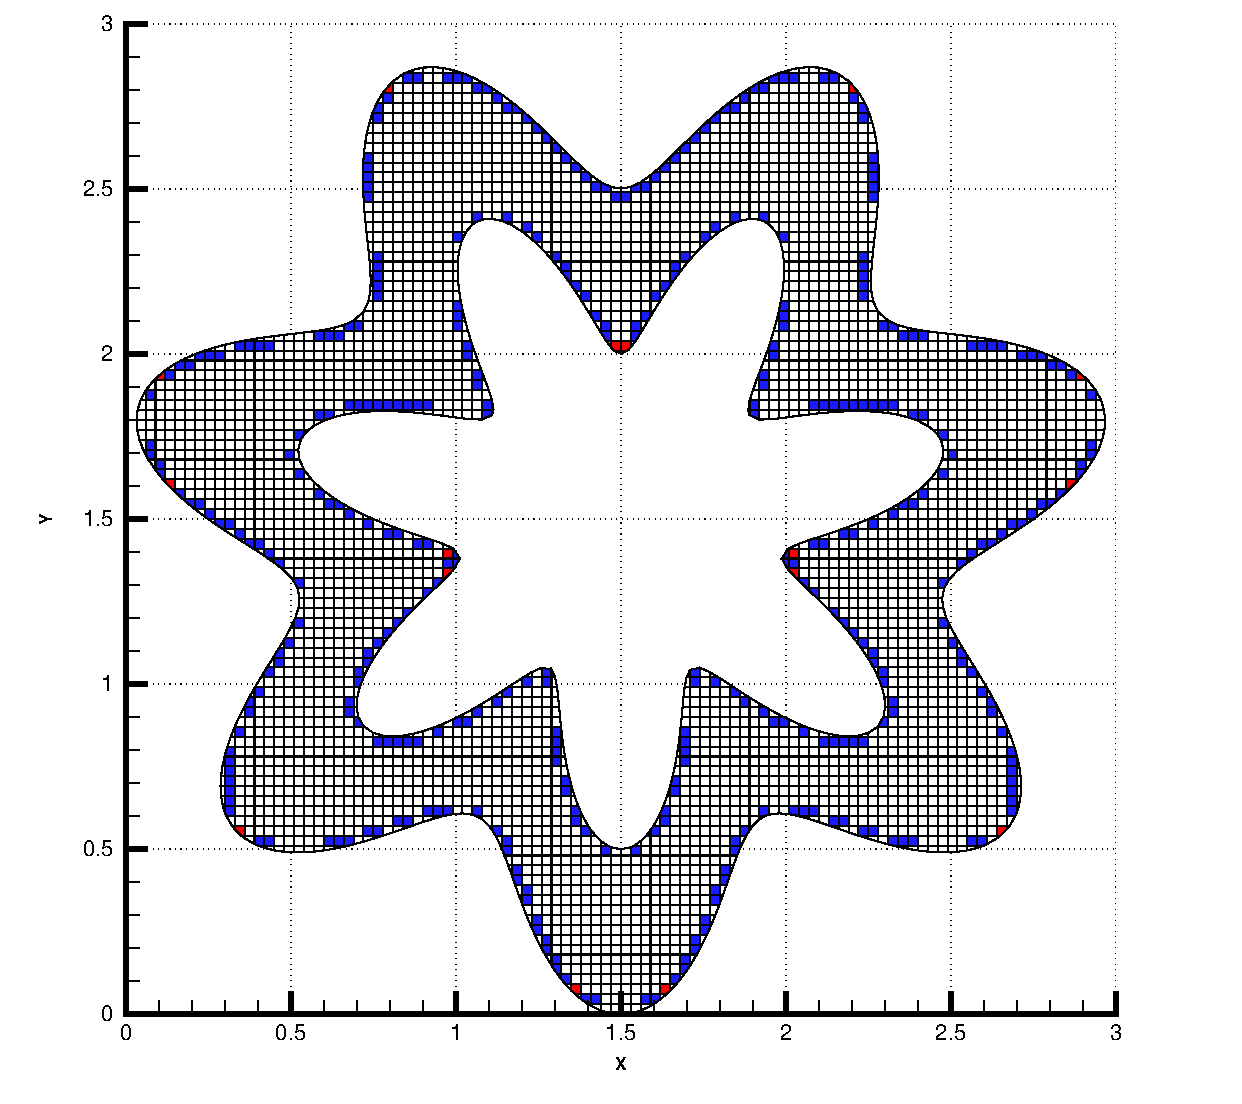
\includegraphics[width=4.5in]{figs/waveynumhoods.eps}
% \caption{\sf Domain from example XX.  Figure shows how many
% neighborhoods each cell belongs to: 
% one (white), two (blue), or three (red).
% The full example is shown in section \ref{sec:compResults}.}
% \label{fig:2nborTile}
% \end{center}
% \end{figure}



%\vspace*{.1in}
\subsection{State redistribution postprocessing} \label{sec:srd_postprocessing}

Once the preprocessing step has been completed, we are able to stabilize the base finite volume scheme after each stage for the method of lines (Section \ref{sec:mol}) or time step for the MUSCL scheme (Section \ref{sec:muscl}). 
In this section, we describe postprocessing on two-dimensional meshes with overlapping neighborhoods, i.e., the analogue of postprocessing on one-dimensional nonuniform grids presented in Section \ref{sec:srd1d}.
%We describe here the two dimensional analogue of Section \ref{sec:srd1d}, which describes postprocessing on a one dimensional nonuniform grid.

%\textit{Note}: we describe here the state redistribution procedure for scalar conservation laws.  The generalization to systems of conservation laws is direct, in that state redistribution can be applied to each component of the vector of conserved quantities independently of one another.

\subsubsection*{Compute the provisionally updated numerical solution}   
Compute one stage or step of one of the finite volume schemes presented in Section \ref{sec:basefv}, i.e.,
\begin{equation} \label{eq:stage_step}
\widehat{U} = U^n + \Delta t  L(U^n),
\end{equation}
where $L$ is the operator in \eqref{eq:molscheme} or \eqref{eq:musclscheme}.  
The update in \eqref{eq:stage_step} corresponds either to one stage for the method of lines or one step of the MUSCL scheme.
$\widehat{U}$ is a vector of provisionally updated, unstable solution averages on the entire grid before state redistribution.

%for the method of lines or in \eqref{eq:musclscheme} for MUSCL. 

%\begin{enumerate}
%\item
\subsubsection*{Compute weighted solution averages on each neighborhood}   

%\vspace*{.1in}
The solution average on each neighborhood is given by
\begin{equation}
\label{tiledef}
\widehat{Q}_{i,j} =  \frac{1}{{\widehat V}_{i,j}} \, \sum_{(r,s) \in M_{i,j}} \,  
\frac{V_{r,s}}{N_{r,s}}  \widehat{U}_{r,s}
\end{equation}
where the volume ${\widehat V}_{i,j}$ is the weighted neighborhood volume defined in \eqref{voldef} and $N_{i,j}$ is the overlap count associated to cell $i,j$ defined in Section \ref{sec:preprocessing}.  
Analogous to the one dimensional case in Section \ref{sec:srd1d}, the weighted solution averages on the merging neighborhood is a convex combination of the provisional solution averages on the neighborhood associated to cell $(i,j)$.  Recall that $M_{i,j}$ is a set of cell indices in the neighborhood of cell $(i,j)$.





%In words, the contribution of each cell is divided by the number of neighborhoods 
%to which is belongs (i.e. its count). 
%Most full cells will have ${\widehat V}_{i,j} = V_{i,j}$, 
%and $\widehat{Q}_{i,j}  = \widehat{U}_{i,j}$, since they have a count of one.
%At the other extreme, if all cells merged with the same number of neighbors, the $N_k$'s
%would cancel, and the resulting solution would be the standard volume-weighted
%solution over the included cells. 

%\item
\subsubsection*{Reconstruct and limit a gradient on each neighborhood}

%\vspace*{.1in}
%All cut cells with area less than $\frac{1}{2} \Delta x \Delta y$ were merged, and will need a
%gradient.
For second order accuracy in space, we compute a gradient on each neighborhood using a least squares procedure.
%A gradient needs to be computed for merging neighborhood. 
%A least squares procedure  similar to the one used in \eqref{eqn:lls} 
%for the finite volume update of the cut cells is an 
%obvious choice.  
%We use a $3 \times 3$ neighborhood around $(i,j)$, ignore solid cells, and fit a least squares solution using the weighted centroids.
The set of merging neighborhood indices using for reconstruction on the neighborhood associated to cell $(i,j)$ is called $\widehat R_{i,j}$.
We note that this set need not be the same as $R_{i,j}$ used in the cut cell gradient reconstruction on the base grid (Section \ref{sec:limit}). 
Similar to the base grid reconstruction in \eqref{eqn:lls}, the reconstruction on neighborhood $(i,j)$ is of the form
\begin{equation}\label{eq:qrecon}
\widehat{q}_{i,j}(x,y) = \widehat{Q}_{i, j} + \widehat{\sigma}_{x,i,j}(x - \widehat{x}_{i,j}) + \widehat{\sigma}_{y,i,j}(y - \widehat{y}_{i,j}),
\end{equation}
where $\widehat{Q}_{i, j}$ is the weighted neighborhood average defined in \eqref{tiledef}, $(\widehat{x}_{i,j},\widehat{y}_{i,j})$ is the weighted centroid of neighborhood $(i,j)$, and $(\widehat{\sigma}_{x,i,j},\widehat{\sigma}_{y,i,j})$ is 
the gradient on the merging neighborhood.
The neighborhood gradient $(\widehat{\sigma}_{x,i,j},\widehat{\sigma}_{y,i,j})$ satisfies in the least squares sense
\begin{equation}\label{eqn:linrecon}
\widehat{\sigma}_{x,i,j}(\widehat{x}_{r,s} - \widehat{x}_{i,j}) +
\widehat{\sigma}_{y,i,j}(\widehat{y}_{r,s} - \widehat{y}_{i,j})=
\widehat{Q}_{r,s} - \widehat{Q}_{i, j} \quad \forall (r,s) \in \widehat{R}_{i,j}.
\end{equation}
Note that \eqref{eqn:linrecon} uses the neighborhood's weighted centroids $(\widehat{x}_{r,s},\widehat{y}_{r,s})$ instead of the cell centroids.  In Section \ref{sec:linex}, we prove that this procedure is linearity preserving.



%The gradient on the merging neighborhood $(\widehat{\sigma}_{x,i,j},\widehat{\sigma}_{y,i,j})$ satisfies in the least squares sense
%\begin{equation}\label{eqn:linrecon}
%\widehat{\sigma}_{x,i,j}(\widehat{x}_{k} - \widehat{x}_{i,j}) + \widehat{\sigma}_{y,i,j}(\widehat{y}_{k} - \widehat{y}_{i,j})= \widehat{Q}_{k} - \widehat{Q}_{i, j} \quad \forall k \in R_{i,j},
%\end{equation}
%where $R_{i,j}$ is the set of indices of neighborhoods used for reconstruction 
%on merging neighborhood $i$.  That is, the reconstruction on the merged neighborhood is the linear function of best fit through the points $(\widehat x_k, \widehat y_k, \widehat Q_k)$ $\forall k \in R_{i,j}$ and that passes exactly through $(\widehat x_{i,j}, \widehat y_{i,j}, \widehat{Q}_{i,j})$.


The set of neighborhoods used for gradient reconstruction on neighborhood $(i,j)$, $\widehat R_{i,j}$, is the $3 \times 3$ tile.
It could happen that this set does not contain enough neighborhoods, or that the weighted centroids of these neighborhoods are too close to compute a well-conditioned gradient.
This is the case in Figure \ref{fig:tooclose}, where the weighted centroids are too close in the $y$ direction.

We remedy this by increasing the stencil size for the gradient computation if the weighted centroids are not at least $\frac{1}{2}\Delta x$  and $\frac{1}{2}\Delta y$ apart in the $x$ or $y$ direction.
For example, if the weighted centroids are too close in the $x$ 
direction, but not the $y$ direction, then the $5\times 3$ tile is used as the 
reconstruction neighborhood.  Similarly, if the weighted centroids are too 
close in the $y$ direction, but not the $x$ direction, then the $3\times 5$ tile is 
used as the reconstruction neighborhood.  The neighborhood size is increased until this distance requirement is satisfied in both $x$ and $y$ directions.  In Figure \ref{fig:tooclose},
the appropriate reconstruction neighborhood is the $3\times 5$ reconstruction tile.

\begin{figure}
    \centering
    \subfloat[The blue merging neighborhood is associated to cut cell $(i,j)$.  The green merging neighborhoods are associated to cut cells $(i-1,j)$ and $(i+1,j)$.]{\includegraphics[width=0.30\linewidth]{figs/tooclose2.pdf} \label{fig:a}} \hfill
    \subfloat[The green merging neighborhoods are associated to the whole cells $(i-1,j+1)$, $(i,j+1)$, and $(i+1,j+1)$.]{\includegraphics[width=0.30\linewidth]{figs/tooclose1.pdf} \label{fig:b}} \hfill
    \subfloat[The weighted centroids of the reconstruction neighborhoods in Figures \ref{fig:a}, \ref{fig:b}.]{\includegraphics[width=0.30\linewidth]{figs/tooclose3.pdf} \label{fig:c}} 
    \caption{\sf 
%    	In (a) and (b), the blue merging neighborhood's $3\times3$ gradient reconstruction 
%    stencil is highlighted in green.
%    On the right, cell $(i,j+1)$ has a stencil highlighted in green, for computing the gradient in $x$. 
    The weighted centroids of the neighborhoods in $\widehat{R}_{i,j}$ are indicated with a cross ($\times$).  
    Here $\widehat{R}_{i,j}$ is the set of merging neighborhoods associated to cells on the $3\times3$ tile centered on cell $(i,j)$.
    Clearly, the weighted centroids are too close to one another in the $y$ direction (Figure \ref{fig:c}).  It follows that least squares system to reconstruct the $x$ and $y$ derivatives of the numerical solution on the blue merging neighborhood is very ill-conditioned.
}
    \label{fig:tooclose}
\end{figure}

%Note that full cells, where the merged  solutions $\widehat{Q}_{i,j} =
%\widehat{U}_{i,j}$ (the
%provisionally updated solution), do not need a gradient. The solution will only be
%evaluated at the cell centroid, which is the same as the neighborhood centroid. 
%Note that the merging neighborhood of the cut cell will
%also contributed to the full cell.

To limit the reconstructed gradient we apply the BJ limiter, this time over $\widehat{R}_{i,j}$ rather than $R_{i,j}$ in \eqref{eqn:bj} and \eqref{eqn:alpha}.  This procedure is linearity preserving since the points to which the neighborhood solutions are reconstructed in \eqref{eq:bj_alpha}, i.e. $(\widehat{x}_{r,s}, \widehat{y}_{r,s})$, are contained in the convex hull of the points at which the minimum and maximums in \eqref{eqn:bj} are computed \cite{giuliani2018analysis}.


\subsubsection*{Final solution update} 
%the average of the reconstructed polynomials that overlap the cell, i.e., the final update for cell $(i,j)$ is

The final update on cell $(i,j)$ is given by 
\begin{equation} \label{eqn:final_update_linear}
U^{n+1}_{i,j} =  \frac{1}{V_{i,j}}\sum_{(r,s) \in W_{i,j}}\frac{1}{N_{i,j}} \int_{\Omega_{i,j}}\widehat q_{r,s}(x,y) ~dx~dy.
\end{equation}
where $W_{i,j}$ is the list of indices of the neighborhoods that overlap cell $(i,j)$ and $N_{i,j}$ is the number of neighborhoods that overlap cell $(i,j)$. 
Since $\widehat{q}_{i,j}(x,y)$ is a linear function, the above simplifies to
\begin{equation} \label{eqn:final_update_linear2}
	U^{n+1}_{i,j} =   \frac{1}{N_{i,j}}\sum_{(r,s)  \in W_{i,j}}\hat{q}_{r,s}(x_{i,j},y_{i,j}),
\end{equation}
i.e., the final update oncell $(i,j)$ is the average of all its neighborhood reconstructions evaluated at $(i,j)$'s physical centroid $(x_{i,j},y_{i,j})$. 


\noindent\textit{Note 1}: when we are stabilizing the method of lines scheme, $U^{n+1}_{i,j}$ corresponds to either the first or second stage of Heun's method, i.e., $U^{(1)}_{i,j}$ or $U^{(2)}_{i,j}$ in \eqref{eq:molscheme}.  
Thus, the method of lines scheme in \eqref{eq:molscheme} when stabilized by state redistribution becomes
\begin{equation}\label{eq:molscheme_srd}
\begin{aligned}
\mathbf{U}^{(1)} &= S(\mathbf{U}^{n} + \Delta t L(\mathbf{U}^n)), \\
\mathbf{U}^{(2)} &= S(\mathbf{U}^{(1)} + \Delta t L(\mathbf{U}^{(1)})), \\
\mathbf{U}^{n+1} &= \frac{1}{2}( \mathbf{U}^{n} + \mathbf{U}^{(2)} ) ,	
\end{aligned}
\end{equation}
where $S$ is the linear state redistribution operator applied after each forward Euler step of Heun's method.
When we are stabilizing the MUSCL scheme $U^{n+1}_{i,j}$ has the same meaning as in \eqref{eq:musclscheme}.  Thus, the MUSCL scheme in \eqref{eq:musclscheme} when stabilized by state redistribution becomes
\begin{equation}\label{eq:musclscheme_srd}
\mathbf{U}^{n+1} = S(\mathbf{U}^{n} + \Delta t L(\mathbf{U}^{n})).
\end{equation}

\noindent\textit{Note 2}: The final update formula \eqref{eqn:final_update_linear} can easily be implemented with a 
nested for loop as in Algorithm \ref{alg:finalupdate}.  This algorithm has the advantage that it does not require computing the set $W_{i,j}$ used in \eqref{eqn:final_update_linear} or \eqref{eqn:final_update_linear2}.  The outer loop iterates over the merging neighborhoods $(i,j)$ and the inner loop iterates over each cell $(r,s)$ in neighborhood $(i,j)$.  Each merging neighborhood $(i,j)$ gives a contribution $ \hat{q}_{i,j}(x_{r,s}, y_{r,s})/N_{r,s} $ to the cells $(r,s)$ that belong to it. 
\begin{algorithm}[H]
		\caption{\sf Final solution update} \label{alg:finalupdate}
	\begin{algorithmic}
	\For{$i,j$}
	\State $U^{n+1}_{i,j} \leftarrow 0$
	\EndFor
	\For{$i,j$}
		\For{$(r,s) \in M_{i,j}$}
			\State $U^{n+1}_{r,s} \leftarrow U^{n+1}_{r,s} + \hat{q}_{i,j}(x_{r,s}, y_{r,s})/N_{r,s} $
		\EndFor
	\EndFor
	\end{algorithmic}
\end{algorithm}


%To use the example of figure \ref{fig:2nborTile}, the cut cell value
%\begin{equation}
%   U_{i,j}^{n+1} := \widehat{Q}_{i,j} 
%   + ( x_{i,j} - \widehat x_{i,j}) \, \widehat{\sigma}_{x,i,j}
%   + ( y_{i,j} - \widehat y_{i,j}) \, \widehat{\sigma}_{y,i,j}
%\end{equation}
%since cell $(i,j)$ only belongs to one neighborhood. The adjacent full cell
%$(i,j+1)$ on the other hand belongs to two neighborhoods -- the one it 
%shares with
%the cut cell $(i,j)$ , and its own merging neighborhood.
%So its solution at time $t^{n+1}$  becomes
%\begin{equation}
%\label{eqn:numhood2ex}
%\begin{split}
%   U_{i,j+1}^{n+1} \,=\, & \frac{1}{2} \, \widehat{q}_{i,j}(x_{i,j+1},y_{i,j+1})+ 
%   \frac{1}{2} \,  \widehat{q}_{i,j+1}(x_{i,j+1},y_{i,j+1}), \\
%   = &\frac{1}{2} \left
%   (\widehat{Q}_{i,j} 
%   + ( x_{i,j+1} - \widehat x_{i,j}) \, \widehat{\sigma}_{x,i,j}
%   + ( y_{i,j+1} - \widehat y_{i,j}) \, \widehat{\sigma}_{y,i,j} \right ) + 
%   \frac{1}{2} \, \widehat{Q}_{i,j+1} .
%\end{split}
%\end{equation}
%The last term  in eq. \eqref{eqn:numhood2ex} has no gradient terms because the
%centroids of the original cell and merged cell are identical.
%The fraction $\frac{1}{2}$ is because cell $(i,j+1)$ is part of  two
%neighborhoods, so each contributes half of the solution.


%One might at first think that only the cut cell need to have its solution replaced
%by the more stable update.  This would not be conservative however; the adjacent cell
%also needs to be part of the update. In addition, each of these cells might also be part of
%another neighborhood if the geometry curves, for example. So in the general case,
%each contribution from a merging tile has to be weighted by the number of
%neigborhoods it contributes to. 






%The conservation properties of the algorithm will be discussed after the
%higher order SRD algorithm is presented in the next
%section. It will also be presented more generally.   

%Different choices of neighborhoods, the minimum volume for the merging
%neighborhood, gradient neighborhoods, and limiting will give
%somewhat different computational results. 
%Some of these will be examined
%theoretically using model problems in one space dimension in section
%\ref{sec:theory}. These choices can affect the stability limit of the
%overall method.
%We will also show computational results using different neighborhood
%choices in section \ref{sec:compResults} in two space dimensions.

\subsection{Linear exactness} \label{sec:linex}
In this section, we show that second order accurate state redistribution preserves linear functions.
Consider the grid function of the numerical solution after one time step
or stage, $\widehat{U}$.  Assume that it can be written in terms of a linear function $f(x,y)$ of the $x$ and $y$ coordinates, i.e.,
\begin{equation}
    \label{eqn:uhatlinear}
\widehat{U}_{i,j} = f(x_{i,j},y_{i,j}) = ax_{i,j} + by_{i,j} + c.
\end{equation}
This assumption is valid since both the method of lines (Section \ref{sec:mol}) and the MUSCL scheme (Section \ref{sec:muscl}) are linearity preserving.  
%That is, after one step or stages of these numerical methods, a linear solution remains linear.
From \eqref{eqn:uhatlinear} and the expression for the average on the merging neighborhood $(i,j)$ in \eqref{tiledef}, we have
\begin{equation}
    \label{eqn:linear1}
\widehat{Q}_{i,j} = \frac{1}{{\widehat V}_{i,j}} \, \sum_{(r,s) \in M_i} \,  
\frac{V_{r,s}}{N_{r,s}}  \,\, (ax_{r,s} + by_{r,s} + c).
\end{equation}
Distributing the summation in \eqref{eqn:linear1}, we have
\begin{equation}\label{eqn:linear2}
\widehat{Q}_{i,j} =  a \left(\frac{1}{{\widehat V}_{i,j}} \, \sum_{(r,s) \in M_{i,j}} \,  
\frac{V_{r,s}}{N_{r,s}} x_{r,s} \right) + b\left(\frac{1}{{\widehat V}_{i,j}} \, \sum_{(r,s) \in M_{i,j}} \,  
\frac{V_{r,s}}{N_{r,s}} y_{r,s} \right) + c\left(\frac{1}{{\widehat V}_{i,j}} \, \sum_{(r,s) \in M_{i,j}} \,
\frac{V_{r,s}}{N_{r,s}}\right) .
\end{equation}
From the definition of the weighted centroid and volume of the merging neighborhood
$(i,j)$ in \eqref{voldef} and \eqref{centroiddef}, respectively, \eqref{eqn:linear2} becomes
\begin{equation}\label{eqn:linear3}
\widehat{Q}_{i,j} =  a \widehat{x}_{i,j} + b\widehat{y}_{i,j} + c = f(\widehat{x}_{i,j},\widehat{y}_{i,j}).
\end{equation}
Now, on neighborhood $(i,j)$, we solve the least squares system in
\eqref{eqn:linrecon} to find $\widehat{\sigma}_{x,i,j}$ and
$\widehat{\sigma}_{y,i,j}$, i.e., the gradient on the merging neighborhood.  Using
\eqref{eqn:linear3} in \eqref{eqn:linrecon}, and due to the linearity of $f$, the following system
\begin{equation}
\widehat{\sigma}_{x,i,j}(\widehat{x}_{r,s} - \widehat{x}_{i,j}) + \widehat{\sigma}_{y,i,j}(\widehat{y}_{r,s} - \widehat{y}_{i,j})= f(\widehat{x}_{r,s}, \widehat{y}_{r,s}) - f(\widehat{x}_{i,j}, \widehat{y}_{i,j}) \quad \forall (r,s) \in \widehat{R}_{i,j},
\end{equation}
is solved exactly by $\widehat{\sigma}_{x,i,j}=a$ and
$\widehat{\sigma}_{y,i,j}=b$.  In other words, the exact gradient 
of $f$ is reconstructed on merging neighborhood $(i,j)$.  
The reconstructed solution is then
\begin{equation}
    \label{eqn:qrecon1}
    \hat{q}_{i,j}(x,y) = f(\widehat{x}_{i,j},\widehat{y}_{i,j}) + a(x-\widehat{x}_{i,j})+b(y-\widehat{y}_{i,j}) .
\end{equation}
Since $f$ is a linear function, \eqref{eqn:qrecon1} becomes
\begin{equation}
    \label{eqn:qrecon2}
    \hat{q}_{i,j}(x,y) = f(x,y).
\end{equation}
By \eqref{eqn:final_update_linear2}, the final solution update is
\begin{equation} 
U^{n+1}_{i,j} = \frac{1}{N_{i,j}}\sum_{(r,s) \in W_{i,j}}f(x_{i,j},y_{i,j}).
\end{equation}
This becomes
\begin{equation} 
U^{n+1}_{i,j} = f(x_{i,j},y_{i,j}),
\end{equation}
i.e., $U^{n+1}_{i,j} = \widehat{U}_{i,j}$, which shows that second order accurate state redistribution is linearity preserving. Numerical experiments in Section \ref{sec:compResults} will demonstrate the scheme's order of accuracy.

%The computational examples will show that the SRD algorithm preserves 
%the accuracy of a second order accurate base scheme. In Section \ref{sec:theory}, we present some analysis that discusses the stability and accuracy of our scheme in one dimension.
%In Section \ref{sec:ho} we will extend both SRD and the RK
%schemes to third order and higher accuracy.





\subsection{Conservation}\label{sec:cons}
%\begin{figure}
%	\centering
%	\includegraphics[width=0.5\textwidth]{figs/simple_example.pdf}
%	\caption{Simple nonuniform grid of three cells where $\Omega_2$ is the small cell and $\Omega_1$ and $\Omega_3$ are large cells.  The red arrows indicate the merging neighborhoods associated to each cell in the grid.}\label{fig:simple_example}
%\end{figure}
In this section, we show that the total mass of the numerical solution before and after state redistribution does not change.  The total mass after state redistribution is 
\begin{equation}\label{eq:total_mass}
\mathcal{M}^{n+1} = \sum_{i,j} V_{i,j} U^{n+1}_{i,j}.
\end{equation}
The above can be written as a sum of mass contributions from each merging neighborhood, i.e.,
\begin{equation}\label{eq:total_mass2}
\mathcal{M}^{n+1} = \sum_{i,j} \widehat{\mathcal{M}}_{i,j},
\end{equation}
where the mass contribution of merging neighborhood $(i,j)$ is
\begin{equation}\label{eq:mi}
\widehat{\mathcal{M}}_{i,j} = \sum_{(r,s) \in M_{i,j}}\frac{1}{N_{r,s}} \int_{\Omega_{r,s}}\widehat q_{i,j}(x,y) ~dx~dy,
\end{equation}
and $\widehat q_{i,j}(x)$ is that neighborhood's polynomial reconstruction defined in \eqref{eq:qrecon}.
Evaluating the integral in \eqref{eq:mi}, we have
\begin{equation}\label{eq:mi1}
\widehat{\mathcal{M}}_{i,j} = \widehat Q_{i,j} \widehat V_{i,j}, 
\end{equation} 
where $\widehat Q_{i,j}$ is the weighted average on neighborhood $(i,j)$.
%Taking into account the linearity of $\widehat{q}_{i,j}(x,y)$, \eqref{eq:mi} can be written
% \begin{equation}\label{eq:mi_lin}
% \widehat{\mathcal{M}}_{i,j} = \sum_{(r,s) \in M_{i,j}}\frac{V_{r,s}}{N_{r,s}} \widehat q_{i,j}(x_{r,s},y_{r,s}),
% \end{equation}
%To illustrate this, consider the simple one dimensional grid in Figure \ref{fig:modelProblem1} composed of seven cells, where $\Omega_{-1}$ and $\Omega_{1}$ are the only small cells.  The red arrows indicate the associated merging neighborhoods, i.e., the merging neighborhood of cell $-1$ comprises $-2$, $-1$, $0$.
%Substituting the final solution update \eqref{eqn:final_update_linear2} into \eqref{eq:total_mass}, the total mass of the numerical solution on this grid at $t^{n+1}$ can be written
%\begin{equation}
%\begin{aligned}
%\mathcal{M}^{n+1} &= V_{-3} \widehat q_{-3}(x_{-3}) + \frac{V_{-2}}{2} \left(  \widehat q_{-2}(x_{-2}) + \widehat q_{-1}(x_{-2}) \right) + V_{-1} \widehat q_{-1}(x_{-1}) \\
%& + \frac{V_0}{3}\left( \widehat q_{-1}(x_0) + \widehat q_{0}(x_0) + \widehat q_{1}(\widehat{x}_0)\right) \\
%&+ V_{1} \widehat q_{1}(x_{1}) + \frac{V_{2}}{2} \left(  \widehat q_{1}(x_{2}) + \widehat q_{2}(x_{2}) \right)  + V_{3} \widehat q_{3}(x_{3}) .
%\end{aligned}
%\end{equation}
%Regrouping terms, the total mass can be rewritten in terms of mass contributions from each merging tile in the form of \eqref{eq:total_mass2} and \eqref{eq:mi}, i.e.,
%\begin{equation}
%\begin{aligned}
%\mathcal{M}^{n+1} = &\underbrace{V_{-3} \widehat q_{-3}(x_{-3}) }_{\widehat{\mathcal{M}}_{-3}} + \underbrace{\frac{1}{2}V_{-2} \widehat q_{-2}(x_{-2})}_{\widehat{\mathcal{M}}_{-2}} \\
%& + \underbrace{\frac{1}{2}V_{-2}\widehat q_{-1}(x_{-2})+V_{-1}\widehat q_{-1}(x_{-1}) + \frac{1}{3}V_{0}\widehat q_{-1}(x_{0})}_{\widehat{\mathcal{M}}_{-1}} +  \underbrace{\frac{1}{3}V_0\widehat q_{0}(x_{0})}_{\widehat{\mathcal{M}}_{0}} \\
%& + \underbrace{\frac{1}{3}V_{0}\widehat q_{1}(x_{0}) + V_{1}\widehat q_{1}(x_{1}) + \frac{1}{2}V_{2}\widehat q_{1}(x_{2})}_{\widehat{\mathcal{M}}_{1}} \\
% & + \underbrace{\frac{1}{2}V_{2} \widehat q_{2}(x_{2})}_{\widehat{\mathcal{M}}_{2}} + \underbrace{V_{3} \widehat q_{3}(x_{3}) }_{\widehat{\mathcal{M}}_{3}} .
%\end{aligned}
%\end{equation}
%Thus, the respective mass contribution of merging neighborhoods 1, 2, and 3, are
%\begin{align*}
%\widehat{\mathcal{M}}_{1} & = \frac{1}{2} \int_{\Omega_1} \widehat q_1(x)~dx, \\
%\widehat{\mathcal{M}}_{2} & =  \frac{1}{2}\int_{\Omega_1} \widehat q_2(x)~dx +  \int_{\Omega_2} \widehat q_2(x)~dx +\frac{1}{2}\int_{\Omega_3} \widehat q_2(x)~dx, \\
%\widehat{\mathcal{M}}_{3} & = \frac{1}{2}\int_{\Omega_3} \widehat q_3(x)~dx.
%\end{align*}
%With the above in mind, we now return to proving mass conservation on a general two dimensional cut cell mesh.
%From the definition of the weighted centroids \eqref{centroiddef} and the linearity of $\widehat{q}_{i,j}$ in \eqref{eq:qrecon}, the mass contribution from an arbitrary merging neighborhood in \eqref{eq:mi_lin} can be written
%\begin{equation*}
%\widehat{\mathcal{M}}_{i,j} = \widehat q_{i,j}(\widehat{x}_{i,j}, \widehat{y}_{i,j}) \widehat V_{i,j},
%\end{equation*}
%i.e.,
%\begin{equation}\label{eq:mi1}
%\widehat{\mathcal{M}}_{i,j} = \widehat Q_{i,j} \widehat V_{i,j}.
%\end{equation}
% \subsection{First order algorithm}
% When $\widehat q_i(x)$ is constant, i.e. $\widehat q_i(x) = \widehat Q_i$ by \eqref{eq:q_avg} and Step 2 in Section \ref{sec:first_order}, \eqref{eq:mi} becomes 
% Substituting \eqref{eq:mi} into \eqref{eq:total_mass2}, we have
% \begin{equation}\label{eq:mi1}
% \widehat{\mathcal{M}}_i = \widehat Q_i \widehat V_i.
% \end{equation}
% by \eqref{eq:q_avg} in the first order algorithm, by \eqref{eq:pq2} in the second order algorithm, and by \eqref{eq:q2} in the third order algorithm.
Using the definition of the weighted average \eqref{tiledef}, the mass contribution from an arbitrary neighborhood \eqref{eq:mi1} becomes
\begin{equation}\label{eq:mi2}
\widehat{\mathcal{M}}_{i,j} = \sum_{(r,s) \in M_{i,j} }\frac{V_{r,s}}{N_{r,s}} \widehat U_{r,s}.
\end{equation}
Substituting \eqref{eq:mi2} into the expression for the total mass in terms of tile contributions \eqref{eq:total_mass2}, the mass at $t^{n+1}$ is
\begin{equation}\label{eq:totalsum}
\mathcal{M}^{n+1} = \sum_{i,j} \sum_{(r,s) \in M_{i,j} }\frac{V_{r,s}}{N_{r,s}} \widehat U_{r,s}.
\end{equation}
Since $N_{r,s}$ indicates the number of times cell $(r,s)$ is overlapped by merging neighborhoods, it follows that the $\frac{V_{r,s}}{N_{r,s}} \widehat U_{r,s}$ term is repeated $N_{r,s}$ times in the sum of \eqref{eq:totalsum}.  Thus, we have that the total mass is
\begin{equation} \label{eq:final}
\mathcal{M}^{n+1} = \sum_{i,j} V_{i,j} \widehat U_{i,j},
\end{equation}
which demonstrates that $\mathcal{M}^{n+1}  = \mathcal{M}^{n}$.

%It may not be immediately obvious how \eqref{eq:totalsum} becomes \eqref{eq:final}, so consider again the simple one dimensional example in Figure \ref{fig:modelProblem1}.  The total mass on this simple grid according to \eqref{eq:totalsum} is
%\begin{equation}
%\begin{aligned}\label{eq:massexample}
%\mathcal{M}^{n+1} = & \underbrace{V_{-3} \widehat U_{-3}}_{\widehat{\mathcal{M}}_{-3}} + \underbrace{\frac{1}{2}V_{-2} \widehat U_{-2} }_{\widehat{\mathcal{M}}_{-2}} + \underbrace{ \frac{V_{-2}}{2}\widehat U_{-2} + V_{-1}\widehat U_{-1} + \frac{V_{0}}{3}\widehat U_{0} }_{\widehat{\mathcal{M}}_{-1}} \\
%&+  \underbrace{\frac{1}{3}V_{0} \widehat U_{0}}_{\widehat{\mathcal{M}}_{0}}  + \underbrace{ \frac{V_{2}}{2}\widehat U_{2} + V_{1}\widehat U_{1} + \frac{V_{0}}{3}\widehat U_{0} }_{\widehat{\mathcal{M}}_{1}}  + \underbrace{\frac{1}{2}V_{2} \widehat U_{2} }_{\widehat{\mathcal{M}}_{2}} + \underbrace{V_{3} \widehat U_{3}}_{\widehat{\mathcal{M}}_{3}}.
%\end{aligned}
%\end{equation}
%Again, $N_{r,s}$ indicates the number of times $\frac{V_{r,s}}{N_{r,s}} \widehat U_{r,s}$ term is repeated in \eqref{eq:totalsum}.  On cell $\Omega_0$, we have $N_0=3$, thus $\frac{V_0}{3} \widehat U_0$ is repeated three times in \eqref{eq:massexample}.  When added together, these three terms become simply $V_0 \widehat U_0$.  The same argument can be applied to the other terms in the sum.  Thus, after simplifying \eqref{eq:massexample}, we have $\mathcal{M}^{n+1} = \mathcal{M}^{n}$.

% The linear advection equation
% $$
% \begin{cases}
%  u_t + a u_x + b u_y = 0 \\
%  u(x,y,0) = f(x,y)
% \end{cases}
% $$
% has the exact solution $u(x,y,t) = f(x-at,y-bt)$.  
% The second order TVD Runge Kutta method stabilized by the SRD method is
% \begin{align}
% U^{(1)} &= ST(U^n + \Delta t L(U^n)),\\
% U^{(2)} &= ST(U^{(1)} + \Delta t L(U^{(1)})),\\
% U^{n+1} &= \frac{1}{2}(U^n + U^{(2)}).
% \end{align}
% The finite volume scheme on the cut cell grid is linearity preserving.  That is, if the initial condition $f$ is a linear function, then the intermediate solution $U^n + \Delta t L(U^n)$ is a grid function of the exact solution at the time $t^n + \Delta t$.  We now must show that the SRD method does not modify this intermediate solution.



%\subsection{Limiting}
%We design a linearity preserving scalar limiter for slopes on the merging neighborhoods.  
%Our goal is to limit the reconstructed gradient on merging neighborhood $i,j$.
%First, we compute the minimum and maximum merging neighborhood average over the reconstruction stencil for the merging neighborhoods $\widehat R_{i,j}$, i.e., 
%\begin{equation}
%     m_{i,j} = \max_{k \in \widehat  R_{i,j}} \widehat{Q}_k \text{ and } M_{i,j} = \max_{k \in R_{i,j}} \widehat{Q}_k.
%\end{equation}
%The reconstructed gradient on merging neighborhood $i,j$ is limited by a nonnegative scalar $\alpha \in [0,1]$, i.e., the limited numerical solution on merging neighborhood $i,j$ is
%\begin{equation}
%    \tilde q_{i,j}(x,y) = \widehat{Q}_{i,j} + \alpha [\widehat{\sigma}_{x,i,j} ( x_{i,j} - \widehat x_{i,j}) \, 
%   + \widehat{\sigma}_{y,i,j}( y_{i,j} - \widehat y_{i,j})],
%\end{equation}
%where $\alpha$ reduces the gradient such that when $\widehat{q}_{i,j}$ is evaluated at the centroids of the neighborhoods in $R_{i,j}$ lies between $m_{i,j}$ and $M_{i,j}$.
%That is, $\alpha$ is given by
%$$
%\alpha = \max\left(0,\min_{k \in R_{i,j}} \alpha_k \right),
%$$
%with
%\begin{equation}
%    \alpha_k = \begin{cases}
%    \frac{\widehat{q}_{i,j}(\widehat x_{k}, \widehat y_{k}) - \widehat{Q}_{i,j}}{M_{i,j} - \widehat{Q}_{i,j}} \text{ if } \widehat{q}_{i,j}(\widehat x_{k}, \widehat y_{k}) - \widehat{Q}_{i,j} \geq 0,\\
%     \frac{\widehat{q}_{i,j}(\widehat x_{k}, \widehat y_{k}) - \widehat{Q}_{i,j}}{m_{i,j} - \widehat{Q}_{i,j}} \text{ if } \widehat{q}_{i,j}(\widehat x_{k}, \widehat y_{k}) - \widehat{Q}_{i,j} < 0.
%    \end{cases}
%\end{equation}
%With this limited gradient, the reconstruction on each merging neighborhood satisfies a local maximum principle
%$$
%m_{i,j} \leq \tilde{q}_{i,j}(\widehat x_k, \widehat y_k) \leq M_{i,j} ~ \forall k \in R_{i,j}.
%$$
%This limiter is linearity preserving since $\tilde{q}_{i,j}$ satisfies a local maximum principle at the points $(\widehat x_k, \widehat y_k) ~\forall k \in R_{i,j}$, which coincide with the points over which $m_{i,j}$ and $M_{i,j}$ are computed [cite lilia and mine JCP paper].
